\chapter{Attack Model}\label{ch:attack}

In this chapter, we will extensively present the threat model of BREACH. We will
explain the conditions that should be met so as to launch the attack and
describe our code implementation for that case. Also, we will investigate the
types of vulnerabilities in web applications that can be exploited with this
attack, as well as introduce alternative secrets, that have not been taken into
consideration before.

\section{Mode of Operation}\label{sec:mo}

\subsection{Description}

The first step of the attack is for the attacker to gain control of the victim's
network, specifically being aple to view the victim's encrypted traffic. This
can be accomplished using the Man-in-the-Middle techniques described in Section
\ref{sec:mitm}.

After that the BREACH JavaScript that issues the requests needs to be executed
from the victim's browser. The first way to do this is to persuade the victim to
visit a website where the js runs, usually with social engineering methods, such
as phishing or spam email. Another way would be for the attacker to inject the
js code in a request made to a regular HTTP website. The following figure
depicts this methodology, which is based on the fact that regular HTTP traffic
is not encrypted and also does not ensure data integrity.

\begin{figure}[H] \caption{JavaScript injection.} \centering
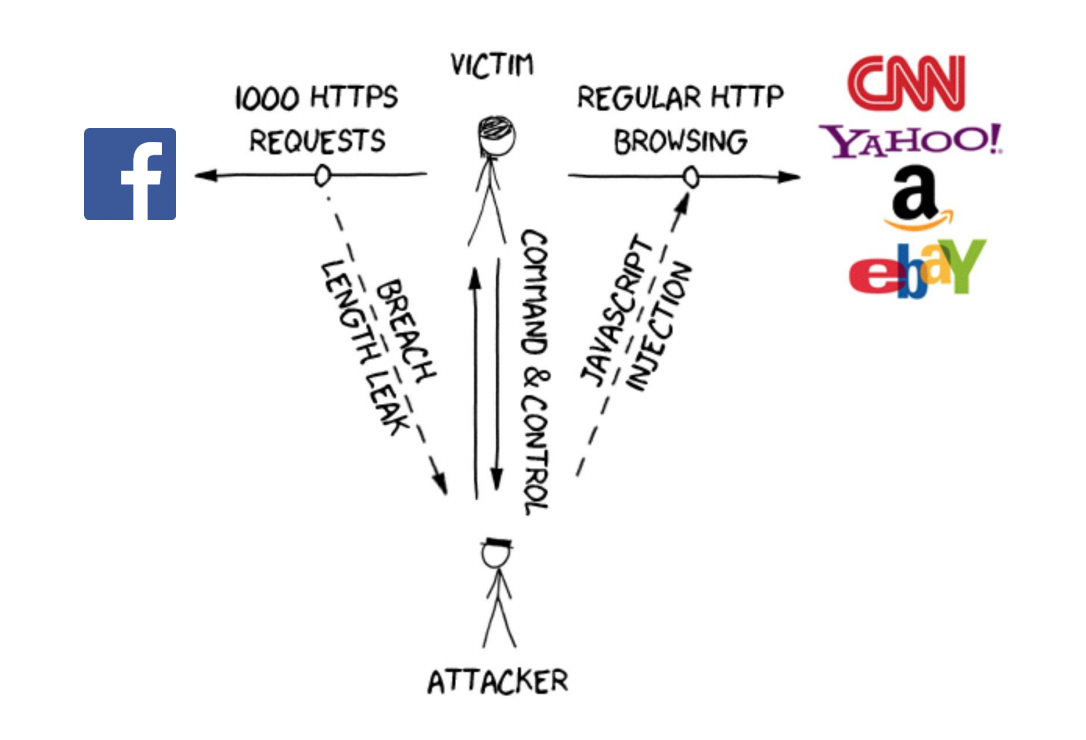
\includegraphics[width=0.6\textwidth]{diagrams/breach_mitm.png}\end{figure}

The script issues multiple requests to the target endpoint, which are sniffed by
the attacker. As described in Section \ref{sec:sameorigin} the attacker cannot
read the plaintext response, however the length of both the request and the
response is visible on the network.

Each request contains some data, that is reflected in the response. Since the
victim is logged in the target endpoint website, the response body will also
contain the secrets. If the conditions defined in Section \ref{subsec:lz77} are
met, the secret and the reflected attacker input will be compressed and
encrypted.

By issuing a large amount of requests for different inputs, the attacker can
analyze the response lengths and extract information about the plaintext
secrets, as described above.

\subsection{Man-in-the-Middle implementation}

In order to gain control of the victim's traffic towards a chosen endpoint, we
created a Python script that performs a Man-in-the-Middle. For the purpose of
this paper, the 'hosts' file of the test machine was configured to redirect
traffic regarding the chosen endpoint towards localhost, as shown below:

\plaintext{Test machine hosts file}{hosts}

The user can set the IPs and ports of the victim and the endpoint, in order for
the Python script to open TCP sockets on both directions, so that traffic from
the victim to the endpoint and vice versa is routed through the
Man-in-the-Middle implementation.

After the environment is set, the script performs an infinite loop, where the
'select' module of Python is used to block the script until a packet is received
on either of the sockets.

If a packet is received, the socket over which it was received can identify the
source of the data. In either case, the packet is parsed in order to log the TLS
header and the payload, after which it is forwarded to the appropriate
destination.

The parser is vital, since header contains information regarding the version of
TLS used, as well as the length of the packet. For that purpose, we have created
a mechanism to perform packet defragmentation, since a TLS record can span over
multiple TCP packets.

Finally, a TLS downgrade attack mechanism is also implemented. In such case, the
Client Hello packet is intercepted and dropped, while the MitM sends as a
response a fatal 'HANDSHAKE FAILURE' alert to the victim.

The victim's browser is usually configured to attempt a connection with a lower
TLS version, where it should also include the "TLS\_FALLBACK\_SCSV" option in the
cipher suite list. If the server is configured properly, the downgrade attempt
should be recognised through the "TLS\_FALLBACK\_SCSV" and the connection should
be dropped. In other case, the TLS version could be downgraded to a point where
a less safe connection is established, such as with version SSL 3.0 or using the
RC4 stream cipher. For further information on the downgrade vulnerabilities see
POODLE \cite{poodle}.

The code described above, as well as the constants library, can be found in
Appendix Sections \ref{sec:connect_py} and \ref{sec:constants_py} respectively.

\subsection{BREACH JavaScript implementation}

For the implementation of the BREACH JavaScript, we assume the user has provided
the alphabet that the secret character belongs to, as well as the known prefix
needed to bootstrap the attack. This information will be written to a file used
by the JavaScript to perform the attack, an example of which is shown below:

\plaintext{request.txt}{request.txt}

The script then uses the jQuery library
\footnote{\url{http://code.jquery.com/jquery-2.1.4.min.js}} to read the info
from the file and begin the attack. If the file is corrupted or either of the
attack variables has changed, a delay of 10 seconds is introduced, so that the
system is balanced. After that, a request for each item of the attack vector is
issued serially, continuing from the beginning when the end of the vector is
reached.

A delay of 10 seconds is also introduced if the above function fails for any
reason, i.e. if the info file does not exist. That way the attack is persistent
and it is the frameworks responsibility to provide the JavaScript with a valid
information file.

For the purpose of this paper, the script was included in a local minimal HTML
web page that was visited in order for the attack to begin. However, with slight
modifications, it could be run on real world applications or injected in HTTP
responses, as described above.

The BREACH script and the HTML web page can be found in the Appendix Sections
\ref{sec:evil_js} and \ref{sec:index_html}.

\section{Vulnerable endpoints}\label{sec:vulnerabilities}

In the original BREACH paper \cite{breach}, Gluck, Harris and Prado investigated
the use of CSRF tokens included in HTTP responses as secrets to be stolen with
the attack. In this paper we suggest alternative secrets, as well as point out
specific vulnerabilities on widely used web applications, such as Facebook and
Gmail.
